\chapter{Speicher-Strukturen} \label{chp:structs}
\epigraph{There are two ways of constructing a software design: One way is to make it so simple that there are obviously no deficiencies, and the other way is to make it so complicated that there are no obvious deficiencies. The first method is far more difficult.}
{C.A.R. Hoare}

Werte im Speicher bilden oft funktionelle Einheiten. In einem Jump'n'Run-Game gehören beispielsweise die x- und y-Koordinate, Blickrichtung sowie die Lebenspunkte der Spielfigur \enquote{zusammen}. Es bietet sich an, Aufgaben wie die Animation beim Laufen, die Überprüfung auf Kollision mit anderen Spielelementen und ähnliches jeweils in Funktionen auszulagern. Diesen Funktionen müssen dann aber jeweils alle genannten Daten als Parameter übergeben werden. Dies kann schnell lästig werden und bietet zusätzlich eine Fehlerquelle, da die Parameter in der richtigen Reihenfolge übergeben werden müssen. An dieser Stelle wollen wir Methoden betrachten, die solche thematischen Einheiten zu kompakten Blöcken zusammen zu fassen.

\section{Sammlungen von Werten: \mintinline{c}{struct}s}
Ein \mintinline{c}{struct} ist ein \emph{selbstdefinierter Datentyp}, in dem mehrere Datensätze zu einem Block zusammengefasst werden. Man kann sich eine \mintinline{c}{struct} also wie eine Sammlung von Tabellenköpfen vorstellen. \mintinline{c}{struct}s haben einen Typen-Namen, sowie für jede Zeile der Tabelle einen Datentyp und einen Feldnamen.

Eine \mintinline{c}{struct} wird folgendermaßen deklariert:
\begin{codebox}[Syntax: Deklaration einer \texttt{struct}]
\begin{minted}{c}
struct Name {
  Datentyp Feldname1;
  Datentyp Feldname2;
  ...
};
\end{minted}
\end{codebox}

Wie üblich ist \texttt{Name} dabei eine alphanumerische Zeichenkette aus bis zu 40 Zeichen, die einen eindeutigen Namen beschreibt, \ie die nicht schon eine Variable im aktuellen Scope oder eine Funktion benennt.

\texttt{Datentyp} ist ein beliebiger Datentyp wie \mintinline{c}{int}, inclusive Pointern oder anderen \mintinline{c}{struct}s.

Die \texttt{Feldname}n sind alphanumerische Zeichenketten von bis zu 40 Zeichen Länge, die jedoch \emph{nicht} global eindeutig sein müssen: eine \mintinline{c}{struct} öffnet ihren eigenen Scope (vgl. die \{geschweiften Klammern\}, in die die Scope-Felder eingeschlossen sind).

Grundsätzlich kann eine \mintinline{c}{struct} an jeder Stelle im Programm angelegt werden; sie ist dann wie gewohnt nur für den aktuellen Scope gültig. Meist wird die Definition einer \mintinline{c}{struct} im gesamten Programm gebraucht; man setzt sie daher üblicherweise global, also vor/außerhalb der \mintinline{c}{main}.

Mit dieser Defintion einer \mintinline{c}{struct} kann man nun Variablen dieses Typs anlegen. Eine Variable eines solchen Typs kann man sich als Spalte einer solchen Tabelle vorstellen. Eine solche Variable wird in einem sinnvollen Scope (\eg in der \texttt{main}) deklariert mit der Syntax:

\begin{codebox}[Syntax: Deklaration einer \texttt{struct}]
\begin{minted}{c}
struct Name Variablenname;
\end{minted}
\end{codebox}

\begin{tcbraster}[raster columns=2,
                  raster equal height,
                  nobeforeafter,
                  raster column skip=0.1cm]
\begin{codebox}[Beispiel: Deklaration einer \texttt{struct}]
\begin{minted}[linenos]{c}
struct Karteieintrag {
  char vorname[50];
  char nachname[50];
  int  geburtsjahr;
  int  geburtsmonat;
  int  geburtstag;
};

int main () {
   struct Karteieintrag Cessi, Chami;
}
\end{minted}
\end{codebox}%
%
\begin{tcolorbox}[title=Visualisierung: Sammlung Tabellenköfpe]
\begin{tabular}{|l|l|l|}
\toprule[1pt]
\emph{Tabellenkopf}		& \texttt{Cessi}	& \texttt{Chami}	\tabcrlf
\texttt{vorname}			& Ce				& Lisl			\tabcrlf
\texttt{nachname}		& Saurus 		& Kohlenstoff	\tabcrlf
\texttt{geburtsjahr}		& 1897			& 1996			\tabcrlf
\texttt{geburtsmonat}	& 9				& 9				\tabcrlf
\texttt{geburtstag}		& 30				& 26				\\
\bottomrule[1pt]
\end{tabular}
\vfill
\end{tcolorbox}
\end{tcbraster}

% include gfx: Rows with type names; 

\subsection{Direkter Zugriff auf \mintinline{c}{struct}-Elemente}
Im obigen Beispiel haben wir die \mintinline{c}{struct} definiert und Variablen des Typs \mintinline{c}{struct Karteieintrag} deklariert. Um nun die einzelnen Felder anzusprechen (\ie die Tabellen-Elemente zu lesen und zu schreiben) bedienen wir uns der Syntax \texttt{Variable.Feldname}. Achten hier auf die Unterscheidung zwischen \emph{Datentyp} (\eg \mintinline{c}{struct Karteieintrag}), \emph{Variable} (\eg \texttt{Cessi}) und \emph{Feldname} (\eg \texttt{vorname}).

\begin{codebox}[Beispiel: Deklaration einer \texttt{struct} und Schreiben in eine \texttt{struct}-Variable]
\begin{minted}[linenos]{c}
#include <string.h>

struct Karteieintrag {                 // Deklaration Datentyp
  char vorname[50];                    // Deklaration Feldelemente
  char nachname[50];
  int  geburtsjahr;
  int  geburtsmonat;
  int  geburtstag;
};

int main () {
  struct Karteieintrag Cessi, Chami;   // Deklaration Variablen
  
  strcpy(Cessi.vorname,  "Ce");        // Zugriffe auf Feldelemente in 'Cessi'
  strcpy(Cessi.nachname, "Saurus");
  Cessi.geburtsjahr  = 1897;
  Cessi.geburtsmonat =    9;
  Cessi.geburtstag   =   30;
\end{minted}
\end{codebox}
\begin{codebox}[]
\begin{minted}[linenos, firstnumber=last]{c}
  strcpy(Chami.vorname,  "Lisl");      // Zugriffe auf Feldelemente in 'Chami'
  strcpy(Chami.nachname, "Kohlenstoff");
  Chami.geburtsjahr  = 1996;
  Chami.geburtsmonat =    9;
  Chami.geburtstag   =   26;
}
\end{minted}
\end{codebox}

Anstatt nun also mit zwei mal fünf getrennten Variablen hantieren zu müssen, können wir nun fünf Werte \enquote{als Paket} behandeln; ein solches Paket darf beispielsweise als Parameter einer Funktion übergeben. Vergleichen Sie die beiden folgenden Funktionen sowie ihre Aufrufe:

\begin{codebox}[Beispiel: Vergleich: Funktion mit \texttt{struct}-Parameter und getrennte Variablen]
\begin{minted}[linenos]{c}
#include <stdio.h>
#include <string.h>

struct Karteieintrag {
  char vorname[50];
  char nachname[50];
  int  geburtsjahr;
  int  geburtsmonat;
  int  geburtstag;
};

void KarteiZeigenGetrennt (
  char vorname[50],
  char nachname[50],
  int  geburtsjahr,
  int  geburtsmonat,
  int  geburtstag
) {
  printf("Vorname:\t%s\n", vorname);
  printf("Nachname:\t%s\n", nachname);
  printf("Geburtstag:\t%04d-%02d-%02d\n",
    geburtsjahr, geburtsmonat, geburtstag
  );
}

void KarteiZeigenStruct (struct Karteieintrag person) {
  printf("Vorname:\t%s\n", person.vorname);
  printf("Nachname:\t%s\n", person.nachname);
  printf("Geburtstag:\t%04d-%02d-%02d\n",
    person.geburtsjahr, person.geburtsmonat, person.geburtstag
  );
}

int main () {
  struct Karteieintrag Cessi, Chami;
  
  /* Eintragen von Werten in Variablen 'Cessi', 'Chami' */
\end{minted}
\end{codebox}
\begin{codebox}[]
\begin{minted}[linenos, firstnumber=last]{c}
  KarteiZeigenGetrennt(
    Cessi.vorname,
    Cessi.nachname,
    Cessi.geburtsjahr,
    Cessi.geburtsmonat,
    Cessi.geburtstag
  );
  
  printf("\n");
  
  KarteiZeigenStruct(Chami); 
}
\end{minted}
\end{codebox}

\begin{cmdbox}[Ausgabebeispiel: Vergleich: Funktion mit \texttt{struct}-Parameter und getrennte Variablen]
\begin{minted}{text}
Vorname:        Ce
Nachname:       Saurus
Geburtstag:     1897-09-30

Vorname:        Lisl
Nachname:       Kohlenstoff
Geburtstag:     1996-09-26
\end{minted}
\end{cmdbox}

Beide Varianten erzeugen eine Ausgabe derselben Form. Bei \texttt{KarteiZeigenGetrennt} müssen jedoch alle fünf Werte im Aufruf getrennt aufgeführt werden (Zeilen 38-44), und erhalten in der Funktionssignatur einen eigenen Eintrag (Zeilen 12-18). Bei der \mintinline{c}{struct}-Version \texttt{KarteiZeigenStruct} dagegen kann der komplette Datensatz \enquote{als Einheit} übergeben werden (Zeile 48). Entsprechend kürzer fällt auch die Funktionssignatur aus (Zeile 26): Hier wird nur eine einzelne Variable \texttt{person} vom Typ \mintinline{c}{struct Karteieintrag} entgegengenommen.

Auch \mintinline{c}{struct}s können ineinander verschachtelt werden:
\begin{codebox}[Beispiel: Verschachtelte Structs]
\begin{minted}[linenos]{c}
struct Datum {
  int  jahr;
  int  monat;
  int  tag;
};

struct Karteieintrag {
  char         vorname[50];
  char         nachname[50];
  struct Datum geburtstag;
};

int main () {
  struct Karteieintrag Tiny;
  Tiny.geburtstag.jahr  = 1994;
  Tiny.geburtstag.monat =    2;
  Tiny.geburtstag.tag   =    3;
}
\end{minted}
\end{codebox}

\subsection{Aliase für Datentypen: \mintinline{c}{typedef}} \label{sec:typedef}
\mintinline{c}{struct}s erlauben zwar bedutend übersichtlichere Strukturen; es wird aber bald lästig, widerholt das Schlüsselwort \mintinline{c}{struct} selbst zu tippen. Aus diesem Grund wird die Deklaration von \mintinline{c}{struct}s häufig mit \mintinline{c}{typedef} verbunden.

\mintinline{c}{typedef} wird benutzt, um zu bestehenden Namen von Datentypen alternative Namen zu definieren (sogenannte \emph{Aliase}). Dies folgt der Syntax:

\begin{codebox}[Syntax: Deklaration einer \texttt{struct}]
\begin{minted}{c}
typedef BezeichnerOriginaltyp Alias;
\end{minted}
\end{codebox}

Sobald auf diese Weise ein \texttt{Alias} definiert ist, kann dieser an jeder Stelle im Code benutzt werden und ersetzt so den gesamten Ausdruck \texttt{BezeichnerOriginaltyp}.

\begin{codebox}[Beispiel: \texttt{typedef} und \texttt{struct}]
\begin{minted}[linenos]{c}
struct Karteieintrag_struct {
  char vorname[50];
  char nachname[50];
  int  geburtsjahr;
  int  geburtsmonat;
  int  geburtstag;
};

typedef struct Karteieintrag_struct Karteieintrag;

int main () {
   Karteieintrag Cessi, Chami;
}
\end{minted}
\end{codebox}

Typedef kann auch für vordefinierte Datentypen benutzt werden, die häufig getippt werden müssen:
\begin{codebox}[Beispiel: \texttt{typedef} und lange Standard-Typen]
\begin{minted}[linenos]{c}
typedef unsigned long long int bignum;
bignum globalvar = 999999999999999999;
\end{minted}
\end{codebox}

Die Definition des Alias \texttt{Karteieintrag} für \mintinline{c}{struct Karteieintrag_struct} erspart in Zeile 12 die Wiederholung des Schlüsselworts \mintinline{c}{struct}; insbesondere gilt das auch für alle weiteren Referenzen auf den Datentyp wie etwa in der Signatur von Funktionen. Neben der Typenbezeichnunt \texttt{Karteieintrag} kann aber auch weiterhin \mintinline{c}{struct Karteieintrag_struct} als Synonym verwendet werden.

Noch kompakter und bequemer wird dies bei der Verwendung von \emph{anonymen \mintinline{c}{struct}s}, also \mintinline{c}{struct}s ohne eigenen Namen. Hier kann die Auflistung der Felder direkt in den \mintinline{c}{typedef}-Befehl mit aufgenommen werden:

\begin{codebox}[Beispiel: \texttt{typedef} und \texttt{struct}]
\begin{minted}[linenos]{c}
typedef struct {
  char vorname[50];
  char nachname[50];
  int  geburtsjahr;
  int  geburtsmonat;
  int  geburtstag;
} Karteieintrag;

int main () {
   Karteieintrag Cessi, Chami;
}
\end{minted}
\end{codebox}

Schließlich ist es auch möglich, im selben Zuge \emph{abgeleitete} Typen zu definieren, \eg einen Pointer auf die soeben definierte \mintinline{c}{struct}:

\begin{codebox}[Beispiel: \texttt{typedef} und \texttt{struct} mit abgeleitetem Typ]
\begin{minted}[linenos]{c}
typedef struct {
  char vorname[50];
  char nachname[50];
  int  geburtsjahr;
  int  geburtsmonat;
  int  geburtstag;
} Karteieintrag, * pKarteieintrag;

int main () {
    Karteieintrag   Cessi;
   pKarteieintrag   CessiRef1 = &Cessi;
    Karteieintrag * CessiRef2 = &Cessi;
}
\end{minted}
\end{codebox}

Durch das \texttt{*} in Zeile 7 wird ausgedrückt, dass das folgende Symbol \texttt{pKarteieintrag} einen Pointer auf die definierte Struktur beschreibt. Folglich wird in Zeile 11 mit \texttt{CessiRef1} eine Variable definiert, die ein Pointer auf \texttt{Karteieintrag} ist. Daneben existiert auch die bereits bekannte Form aus Zeile 12. Die Variablen \texttt{CessiRef1} und \texttt{CessiRef2} haben also denselben Datentyp.

\begin{hintbox}[Sinn und Unsinn von \texttt{typedef}s]
Die Möglichkeit, mit \mintinline{c}{typedef} kürzere Aliase für unhandliche Ausdrücke einzuführen birgt die Gefahr, sich in einem undurchsichtigen Gewirr von Definitionen zu verstricken. Gerade wenn von \mintinline{c}{typedef}s noch andere Typen abgeleitet werden, ist es oft schwer, die \enquote{Verwandtschaftsbeziehungen} noch nachzuvollziehen und sinnvollen Code zu schreiben.

Nach meiner Erfahrung gibt es zwei Situationen, in denen \mintinline{c}{typedef} die Arbeit in C tatsächlich leichter macht:
\begin{itemize}
\item \mintinline{c}{struct}s sowie Pointer auf \mintinline{c}{struct}s, so wie oben gezeigt
\item Funktionszeiger, wie wir sie in Abschnitt \ref{sec:funcPtr} kennengelernt haben.
Die reine Umdefinition bestehender Typennamen dagegen sollte eher vermieden werden.
\end{itemize}
\end{hintbox}

\begin{hintbox}[]
Im Kontext von Funktionszeigern macht die Verwendung von \mintinline{c}{typedef} den Code nicht nur kürzer, sondern bedeutend intuitiver lesbar (sofern man sprechende Typennamen definiert). Sehen Sie folgendes Beispiel an:

\begin{codebox}[\texttt{typedef} und Funktionszeiger]
\begin{minted}{c}
typedef int (*funcPtr_comp) (const void *, const void *);

/* Originaldefintion wie von der cpp-Referenz
 * void qsort( void * ptr, size_t count, size_t size,
 *             int (*comp)(const void *, const void *) );
 */
void qsort (void * ptr, size_t count, size_t size, 
            funcPtr_comp comp);
\end{minted}
\end{codebox}
Die Originaldefinition erlaubt zwar, direkt Rückgabetyp und Typ der Parameter zu entnehmen; es ist aber schwierig, hier auf einen Blick zu erfassen, welches der Name des Parameters ist, und was zur Beschreibung des Typs gehört. In der zweiten Version wird vorausgesetzt, dass der/die ProgrammiererIn die Signatur von \texttt{comp} kennt; dafür wird die Signatur von \texttt{qsort} übersichtlich und entspricht eher einer menschlichen Gedankeneinheit. Die Meinungen hierzu gehen bisweilen aber weit auseinander.
\end{hintbox}

\mintinline{c}{struct}s können auch Pointer auf Instanzen desselben Typs enthalten:
\begin{codebox}[Beispiel: \texttt{struct} mit Referenz auf Instanz gleichen Typs]
\begin{minted}[linenos]{c}
struct linkedList{
  double              content;
  struct linkedList * next;
};
\end{minted}
\end{codebox}

Während das Symbol \mintinline{c}{struct linkedList} schon \enquote{in der Definition der \mintinline{c}{struct}} zur Verfügung steht, sind mit \mintinline{c}{typdef} definierte Symbole erst \emph{nach Abschluss} des Befehls verwendbar:

\begin{warnbox}[Beispiel: \texttt{typedef} und \texttt{struct} mit Referenz auf Instanz gleichen Typs (fehlerhaft), leftupper=7mm]
\begin{minted}[linenos]{c}
typedef struct {
  double       content;
  // linkedList * next;   // Fehler: linkedList noch nicht definiert
} linkedList;
\end{minted}
\end{warnbox}

Um für solche Strukturen dennoch den Komfort von \mintinline{c}{typedef} nutzen zu können, arbeitet man hier mit \emph{benannten \mintinline{c}{struct}s} (im Gegensatz zu \emph{anonymen \mintinline{c}{struct}s}):

\begin{codebox}[Beispiel: \texttt{typedef} und \texttt{struct} mit Referenz auf Instanz gleichen Typs (korrekt)]
\begin{minted}[linenos]{c}
typedef struct LL_struct {
  double             content;
  struct LL_struct * next;   // okay: struct LL_struct kann aufgelöst werden
} linkedList;                // Symbol linkedList steht ab hier zur Verfügung.
\end{minted}
\end{codebox}

In Kapitel \ref{chp:linkedlist} werden wir uns ausführlicher mit solchen Strukturen beschäftigen.

\subsection{\mintinline{c}{struct}s und Pointer}
Wie Sie bereits festgestellt haben, müssen wir in C häufig mit Pointern arbeiten. Im vorigen Abschnitt wurden bereits Pointer auf \mintinline{c}{struct}s angesprochen. Dazu sei hier zuerst ein Syntaxelement vorgestellt, und weiter einige Beispiele besprochen:

\subsubsection{Kombinierter Pointer-Feldzugriffs-Operator}
Haben wir einen Pointer auf eine \mintinline{c}{struct}, so muss für einen Feldzugriff der Pointer zuerst dereferenziert (Operator \texttt{*}) werden und anschließend das angesprochene Feld über den Feldzugriffoperator (\texttt{.}) ausgewählt werden. Da der Feldzugriffsoperator eine höhere Präzedenz hat als die Dereferenzierung (\ie \texttt{.} wird vor \texttt{*} ausgewertet; siehe Tabelle \ref{tab:OperatorPrecedence}), muss mit Klammern gearbeitet werden:

\begin{codebox}[Beispiel: Dereferenzierung und Feldzugriff]
\begin{minted}[linenos]{c}
/* Definition von Karteieintrag und pKarteieintrag wie im vorigen Kapitel */
int main () {
   Karteieintrag        Tiny;
  pKarteieintrag ptr = &Tiny;
  
  printf("Jahr: %4d\n", (*ptr).geburtsjahr);
}
\end{minted}
\end{codebox}

Diese umständliche Form kann durch den kombinierten \emph{Pointer-Feldzugriffs-Operator} \texttt{->} ersetzt werden:

\begin{codebox}[Beispiel: kombinierter Operator]
\begin{minted}[linenos]{c}
/* Definition von Karteieintrag und pKarteieintrag wie im vorigen Kapitel */
int main () {
   Karteieintrag        Tiny;
  pKarteieintrag ptr = &Tiny;
  
  printf("Jahr: %4d\n", ptr->geburtsjahr);
}
\end{minted}
\end{codebox}

\subsubsection{Pointer als Feldelemente}
Selbstverständlich können auch die Feldelemente einer \mintinline{c}{struct} selbst Pointer enthalten. In den obigen Beispielen etwa sind \texttt{vorname} und \texttt{nachname} \mintinline{c}{char}-Arrays und damit Pointer. Der Dereferenzierungs-Operator \texttt{*} wirkt in diesem Fall auf das Feldelement:
\begin{codebox}[Beispiel: Zugriff auf Pointer-Feldelemente (1)]
\begin{minted}[linenos]{c}
/* Definition von Karteieintrag und pKarteieintrag wie im vorigen Kapitel */
int main () {
  Karteieintrag Tiny;
  
  printf("Erster Buchstabe von Tinys Vornamen: %c\n", *Tiny.vorname);
}
\end{minted}
\end{codebox}

Ebenso verhält es sich mit dem Array-Index-Zugriffsoperator \texttt{[]}:
\begin{codebox}[Beispiel: Zugriff auf Pointer-Feldelemente (2)]
\begin{minted}[linenos]{c}
/* Definition von Karteieintrag und pKarteieintrag wie im vorigen Kapitel */
int main () {
  Karteieintrag        Tiny;
  
  printf("Erster Buchstabe von Tinys Vornamen: %c\n", Tiny.vorname[0]);
}
\end{minted}
\end{codebox}

\subsubsection{Pointer in Basis-Variable und in den Feldelementen}
Ist die Variable, über die die \mintinline{c}{struct} angesprochen wird, selbst eine Pointer-Variable, so wird der kombinierte Pointer-Feldzugriffs-Operator \texttt{->} zuerst aufgelöst; anschließend wirken \texttt{*} bzw \texttt{[]}:

\begin{codebox}[Beispiel: kombinierter Operator und Pointer-Feldelemente]
\begin{minted}[linenos]{c}
/* Definition von Karteieintrag und pKarteieintrag wie im vorigen Kapitel */
int main () {
   Karteieintrag        Tiny;
  pKarteieintrag ptr = &Tiny;
  
  printf("Erster Buchstabe von Tinys Vornamen: %c\n", *ptr->vorname   );
  printf("Erster Buchstabe von Tinys Vornamen: %c\n",  ptr->vorname[0]);
}
\end{minted}
\end{codebox}

Siehe hierzu auch Tabelle \ref{tab:OperatorPrecedence}.

\subsubsection{Arrays von Structs}
Man kann auch \emph{Arrays von \mintinline{c}{struct}s} anlegen. In diesem Fall setzt man den Array-Zugriffsoperator \texttt{[]} an die Array-Variable. Unabhängig davon können weiter Operationen auf Array-Feldelemente durchgeführt werden:

\begin{codebox}[Beispiel: Array von \texttt{struct}s]
\begin{minted}[linenos]{c}
typedef struct {
  char vorname[50];
  char nachname[50];
  int  geburtsjahr;
  int  geburtsmonat;
  int  geburtstag;
} Karteieintrag, * pKarteieintrag;
\end{minted}
\end{codebox}
%
\begin{codebox}[]
\begin{minted}[linenos, firstnumber=last]{c}
int main () {
  Karteieintrag listeGeburtstage[3];

  strcpy(listeGeburtstage[0].vorname,  "Ce");
  strcpy(listeGeburtstage[0].nachname, "Saurus");
  listeGeburtstage[0].geburtsjahr  = 1897;
  listeGeburtstage[0].geburtsmonat =    9;
  listeGeburtstage[0].geburtstag   =   30;
  
  strcpy(listeGeburtstage[1].vorname,  "Lisl");
  strcpy(listeGeburtstage[1].nachname, "Kohlenstoff");
  listeGeburtstage[1].geburtsjahr  = 1996;
  listeGeburtstage[1].geburtsmonat =    9;
  listeGeburtstage[1].geburtstag   =   26;
  
  strcpy(listeGeburtstage[2].vorname,  "Tiny");
  strcpy(listeGeburtstage[2].nachname, "Mürrisch");
  listeGeburtstage[2].geburtsjahr  = 1994;
  listeGeburtstage[2].geburtsmonat =    2;
  listeGeburtstage[2].geburtstag   =    3;
    
  printf("Erster Buchstabe Vorname 3: %c\n", *listeGeburtstage[2].vorname    );
  printf("Erster Buchstabe Vorname 3: %c\n",  listeGeburtstage[2]->vorname[0]);
}
\end{minted}
\end{codebox}

Machen Sie sich hier nochmal die Bedeutung der einzelnen Symbole klar:
\begin{itemize}
\item \texttt{Karteieintrag} ist ein \emph{Datentyp} und beschreibt nur die Struktur einer Variable; das
	Symbol selbst beschreibt aber keine Werte.
\item \texttt{pKarteieintrag} ist ebenfalls ein \emph{Datentyp}. Er beschreibt aber keine 
	\mintinline{c}{struct}, sondern einen \emph{Pointer} darauf, \ie die Information, wo im Speicher die
	tatsächliche Instanz der \mintinline{c}{struct} zu finden ist. Verbunden mit dieser Adresse ist die
	Information,  welche Art von Werten an der angegebenen Speicherstelle zu finden sind -- eben die 
	\mintinline{c}{struct} \texttt{Karteieintrag}.
\item \texttt{geburtstag} ist ein Element der \mintinline{c}{struct Karteieintrag}, und damit ohne
	Kontext ein nicht deklariertes Symbol. Nur in Verwendung mit Instanzen von \texttt{Karteieintrag}
	kann dieses Symbol gebraucht werden.
\item \texttt{listeGeburtstage} ist ein Array vom Typ \texttt{Karteieintrag} und damit eine Variable vom
	Typ \texttt{pKarteieintrag}. In dieser Variablen ist nur eine Zahl gespeichert, die die Adresse des 
	ersten Elements des Arrays im Speicher angibt.
\item \texttt{listeGeburtstage[0]} ist nun tatsächlich ein Objekt vom Typ \texttt{Karteieintrag}, \ie
	eine Sammlung von fünf Variablen. Man spricht auch von einer \emph{Instanz} von
	\texttt{Karteieintrag}. Es handelt sich um das erste Element der Liste. Dieser Ausdruck kann \eg an
	Funktionen übergeben werden, die als Argument ein Objekt vom Typ \texttt{Karteieintrag} erwarten 
	(wie im vorigen \emph{Beispiel: Vergleich: Funktion mit \texttt{struct}-Parameter und getrennte
	 Variablen} die Funktion \texttt{KarteiZeigenStruct}.)
\item \texttt{listeGeburtstage[1].geburtsjahr} ist ein \mintinline{c}{int}-Wert. Er gehört zu der
	Instanz 	\texttt{listeGeburtstage[1]}, also zur zweiten Instanz des Typs \texttt{Karteieintrag} im
	Array.
\item \texttt{listeGeburtstage[2].vorname} ist ein \texttt{char *}, der zum dritten Element des Arrays
	\texttt{listeGeburtstage} gehört.
\item \texttt{*listeGeburtstage[2].vorname} ist die Dereferenzierung des oben genannten Objekts, und
	damit ein \mintinline{c}{char}.
\item \texttt{listeGeburtstage->geburtstag} ist gleichbedeutend mit
	\texttt{(*listeGeburtstage).geburtstag} oder \texttt{listeGeburtstage[0].geburtstag}. Es handelt
	sich um einen \mintinline{c}{int}-Wert, der zum ersten Element des Arrays gehört.
\item \texttt{listeGeburtstage[3]} ist ein Verweis auf das vierte Element des Arrays, das aber nicht
	existiert. Es handelt sich hierbei also um eine fehlerhafte Referenz.
\end{itemize}

\subsection{\mintinline{c}{struct}s im Speicher}
Wir können uns Instanzen von \mintinline{c}{struct}s ähnlich vorstellen wie Arrays. Im Unterschied zu diesen werden die einzelnen Elemente nicht über einen \emph{Index} angesprochen, sondern über einen \emph{Feldnamen}. Außerdem haben die einzelnen Elemente nicht  denselben Datentyp. Im Grunde aber wird dieselbe Speicherstruktur angelegt:

\begin{tcolorbox}[title=Speicherbild]
\begin{center}
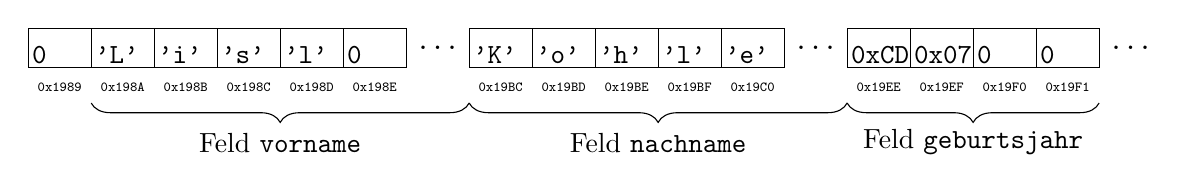
\begin{tikzpicture}
  [ 
    cell/.style={
       text width =7mm,
       text height=4mm, 
       draw=black, 
       inner sep=0.5mm
    },
    ld/.style={
       draw=blue,
       shorten >=2pt,
       ->
    }
  ]
  \node (c00) at ( 0.0,1) [cell] {\ttfamily  0 };
  \node (c01) at ( 0.8,1) [cell] {\ttfamily 'L'};
  \node (c02) at ( 1.6,1) [cell] {\ttfamily 'i'};
  \node (c03) at ( 2.4,1) [cell] {\ttfamily 's'};
  \node (c04) at ( 3.2,1) [cell] {\ttfamily 'l'};
  \node (c05) at ( 4.0,1) [cell] {\ttfamily  0 };
  \node (c06) at ( 4.8,1)        {\ttfamily \ldots};
  \node (c07) at ( 5.6,1) [cell] {\ttfamily 'K'};
  \node (c08) at ( 6.4,1) [cell] {\ttfamily 'o'};
  \node (c09) at ( 7.2,1) [cell] {\ttfamily 'h'};
  \node (c10) at ( 8.0,1) [cell] {\ttfamily 'l'};
  \node (c11) at ( 8.8,1) [cell] {\ttfamily 'e'};
  \node (c12) at ( 9.6,1)        {\ttfamily ...};
  \node (c13) at (10.4,1) [cell] {\ttfamily 0xCD};
  \node (c14) at (11.2,1) [cell] {\ttfamily 0x07};
  \node (c15) at (12.0,1) [cell] {\ttfamily  0 };
  \node (c16) at (12.8,1) [cell] {\ttfamily  0 };
  \node (c17) at (13.6,1)        {\ttfamily ...};

  \node (p00) at ( 0.0,0.5)      {\ttfamily \tiny 0x1989};
  \node (p01) at ( 0.8,0.5)      {\ttfamily \tiny 0x198A};
  \node (p02) at ( 1.6,0.5)      {\ttfamily \tiny 0x198B};
  \node (p03) at ( 2.4,0.5)      {\ttfamily \tiny 0x198C};
  \node (p04) at ( 3.2,0.5)      {\ttfamily \tiny 0x198D};
  \node (p05) at ( 4.0,0.5)      {\ttfamily \tiny 0x198E};
  
  \node (p06) at ( 5.6,0.5)      {\ttfamily \tiny 0x19BC};
  \node (p06) at ( 6.4,0.5)      {\ttfamily \tiny 0x19BD};
  \node (p06) at ( 7.2,0.5)      {\ttfamily \tiny 0x19BE};
  \node (p06) at ( 8.0,0.5)      {\ttfamily \tiny 0x19BF};
  \node (p06) at ( 8.8,0.5)      {\ttfamily \tiny 0x19C0};
  
  \node (p06) at (10.4,0.5)      {\ttfamily \tiny 0x19EE};
  \node (p06) at (11.2,0.5)      {\ttfamily \tiny 0x19EF};
  \node (p06) at (12.0,0.5)      {\ttfamily \tiny 0x19F0};
  \node (p06) at (12.8,0.5)      {\ttfamily \tiny 0x19F1};
  
  \draw [decorate, decoration={brace,amplitude=7pt, mirror}, xshift=-0pt, yshift=0pt]
  		( 0.4, 0.3) -- ( 5.2, 0.3) node [midway, yshift=-0.5cm] 
		(braceArrayPreResize) {Feld \texttt{vorname}};

  \draw [decorate, decoration={brace,amplitude=7pt, mirror}, xshift=-0pt, yshift=0pt]
  		( 5.2, 0.3) -- (10.0, 0.3) node [midway, yshift=-0.5cm] 
		(braceArrayPreResize) {Feld \texttt{nachname}};

  \draw [decorate, decoration={brace,amplitude=7pt, mirror}, xshift=-0pt, yshift=0pt]
  		(10.0, 0.3) -- (13.2, 0.3) node [midway, yshift=-0.5cm] 
		(braceArrayPreResize) {Feld \texttt{geburtsjahr}};		
\end{tikzpicture}
\end{center}
\end{tcolorbox}

Da \mintinline{c}{struct}s einen Datentyp definieren, kann mit \mintinline{c}{sizeof} der Speicherbedarf \emph{einer Instanz} ermittelt werden. Es handelt sich dabei um die Summe der Speicherbedarfe der einzelnen Elemente:

\begin{codebox}[Beispiel: \texttt{sizeof} und \texttt{struct}]
\begin{minted}[linenos]{c}
struct Karteieintrag {
  char vorname[50];
  char nachname[50];
  int  geburtsjahr;
  int  geburtsmonat;
  int  geburtstag;
};

int main () {
  struct Karteieintrag Tiny;
  
  printf("%lu\n", sizeof(Karteieintrag));
  printf("%lu\n", sizeof(Tiny));
}
\end{minted}
\end{codebox}

\begin{cmdbox}[Ausgabebeispiel: \texttt{sizeof} und \texttt{struct}]
\begin{minted}{text}
112
112
\end{minted}
\end{cmdbox}

Diese 112 Bytes pro \texttt{Karteieintrag} kommen aus jeweils 50 Bytes für die beiden \mintinline{c}{char}-Arrays \texttt{vorname} und \texttt{nachname} zusammen sowie dreimal 4 Bytes für die \mintinline{c}{int}s \texttt{geburtsjahr}, \texttt{geburtsmonat} und \texttt{geburtstag}.

\subsection{Operationen mit \mintinline{c}{struct}s}
Während viele Rechenoperationen mit \mintinline{c}{struct}s \emph{denkbar} sind, ist in C nur die Wertzuweisung \texttt{=} definiert. Der Grund hierfür ist, dass für zusammengesetzte Typen nicht eindeutig ist, wie etwa eine Addition stattfinden soll, oder nach welchen Kriterien entschieden wird, welche Instanz \enquote{größer als} eine andere ist. Wo solche Aufgaben gelöst werden sollen, schreibt man Funktionen:

\begin{codebox}[Beispiel: \texttt{sizeof} und \texttt{struct}]
\begin{minted}[linenos]{c}
#include <stdio.h>
#include <math.h>

typedef struct {
  double x;
  double y;
} Punkt2D;

int vergleichPunkt2D (Punkt2D a, Punkt2D b) {
  /* Vergleich nach Kriterium 'Entfernung zum Nullpunkt' 
   * Rückgabewerte:
   *  0, wenn a und b gleich weit entfernt
   * -1, wenn a näher am Nullpunkt als b
   * +1, wenn b näher am Nullpunkt als a
   */
  
  double la = hypot(a.x, a.y),   // hypot: definiert in math.h
         lb = hypot(b.x, b.y);   // berechnet sqrt(a.x * a.x  +  b.x * b.x)
  
  if (la == lb) {return 0;}
  else          {return la < lb  ?  -1  :  +1;}
}

int main () {
  Punkt2D a = {5.0, 5.0}, b = a;
  printf("%d\n", vergleichPunkt2D(a, b));
  // printf("%d\n" a == b); Fehler: kein direkter Vergleich von struct-Instanzen
}
\end{minted}
\end{codebox}

\subsection{Initializer-Syntax} \label{sec:structInit}
Ähnlich wie bei Arrays können \mintinline{c}{struct}-Instanzen bei der Deklaration gleich Werte zugewiesen werden, indem wir diese in \{geschweiften Klammern\} aufführen:

\begin{codebox}[Beispiel: Initializer-Syntax bei \texttt{struct}s]
\begin{minted}[linenos]{c}
typedef struct {
  int  jahr;
  int  monat;
  int  tag;
} Datum;

int main () {
  Datum tag = {1989, 3, 29};
}
\end{minted}
\end{codebox}

Diese Kurzform ist jedoch \emph{ausschließlich} bei der Deklaration von \mintinline{c}{struct}-Instanzen zulässig. Im folgenden Beispiel sind Deklaration und Wertzuweisung getrennt; daher funktioniert dort die Initializer-Syntax nicht mehr:

\begin{codebox}[Beispiel: Initializer-Syntax bei \texttt{struct}s]
\begin{minted}[linenos]{c}
typedef struct {
  int  jahr;
  int  monat;
  int  tag;
} Datum;

int main () {
  Datum tag;
  // tag = {1989, 3, 29};  Fehler: Initiaizer-Syntax außerhalb von Deklaration
}
\end{minted}
\end{codebox}

Dies liegt daran, dass mit diesem abhängig vom Kontext sehr unterschiedliche Ergebnisse erzielt werden. Enthält die \mintinline{c}{struct} ein \mintinline{c}{char}-Array fester Größe (wie im obigen Beispiel das \mintinline{c}{struct Karteieintrag}: Die Felder \mintinline{c}{vorname} und \mintinline{c}{nachname} sind beide \mintinline{c}{char}-Arrays der Größe \texttt{50}), so wird ein String-Literal (ein Ausdrucke in \texttt{"}doppelten Anführungszeichen\texttt{"}) direkt in das Array kopiert; allgemeinen Pointern dagegen wird die Adresse des Literals selbst zugewisen.

\begin{codebox}[Beispiel: Initializer-Syntax bei Strings]
\begin{minted}[linenos]{c}
#include <stdio.h>
#include <stdlib.h>

typedef struct {
  char   constSizeArray[50];
  char * charPointer;
} twoStrings;
\end{minted}
\end{codebox}
%
\begin{codebox}[]
\begin{minted}[linenos, firstnumber=last]{c}
int main () {
  twoStrings x = {"Pure Vernunft Darf Niemals Siegen",   // constSizeArray
                  "Pure Vernunft Darf Niemals Siegen"};  // charPointer
  
  printf("Startadresse der Instanz:\t%p\n"  , (void *)(&x));
  printf("Adresse von constSizeArray:\t%p\n", (void *)(x.constSizeArray));
  printf("Adresse von charPointer:\t%p\n",    (void *)(x.charPointer));
}
\end{minted}
\end{codebox}

\begin{cmdbox}[Ausgabebeispiel: Initializer-Syntax bei Strings]
\begin{minted}{text}
Startadresse der Instanz:       0x7ffc0d4172c0
Adresse von constSizeArray:     0x7ffc0d4172c0
Adresse von charPointer:        0x562bd763b808
\end{minted}
\end{cmdbox}

Das erste String Literal (Zeile 9) soll dem Feld \texttt{constSizeArray} zugewiesen werden, für das ab Beginn der \mintinline{c}{struct}-Instanz 50 Byte frei gehalten werden. Die Zeichenkette wird auf genau diese Speicherstelle kopiert. In den Zeilen 12 und 13 wird daher auch dieselbe Adresse für \texttt{\&x} (die Adresse der Instanz \texttt{x}) und für \texttt{x.constSizeArray} (die Adresse des \mintinline{c}{char}-Arrays \texttt{x.constSizeArray}) ausgegeben. Zeiel 14 nennt dagegen eine ganz andere Adresse, da für das Feld \texttt{charPointer} lediglich eine Adresse speichert, nicht aber den String selbst. Entsprechend wird hier die \emph{Adresse des String-Literals} abgelegt; wir können uns dies vorstellen als \emph{die Adresse des String-Literals im Code}.

Diese letzten Überlegungen waren vermutlich schwer zu verfolgen; bitte entnehmen Sie diesem Abschnitt, dass die Initializer-Syntax im allgemeinen eine schnelle Wertzuweisung zu \mintinline{c}{struct}-Instanzen erlaubt, dass aber beim Umgang mit Arrays Vorsicht geboten ist. Wo Sie sich nicht sicher sind, können Sie jederzeit die zuerst gezeigten expliziten Wertzuweisungen benutzen.

\section{Casting-Interface: \mintinline{c}{union}s}
\mintinline{c}{union}s sind \mintinline{c}{struct}s, bei denen alle Felder auf dieselbe Speicheradresse gelegt werden. Das bedeutet, dass man über verschiedene Bezeichner dieselben Werte bearbeiten kann. Dies kann für manche Elektronik-Anwendungen nützlich sein, in denen Datenpakete in anderen \enquote{Einheiten} versandt und empfangen werden als sie das Steuerprogramm verarbeitet.

Beispiel: Im folgenden Beispiel wird einem \mintinline{c}{int} ein \mintinline{c}{char}-Array überlagert:

\begin{codebox}[Beispiel: \texttt{union} aus \texttt{int} und \texttt{char}s]
\begin{minted}[linenos]{c}
#include <stdio.h>

typedef union {
  int  i;
  char c[4];
} intUnion;

int main () {
  intUnion u;
  
  for (int i=254; i<260; i++) {
    u.i = i;
    
    printf("Integer: %d\n", u.i);
    for (int n=0; n<4; n++) {
       printf("  Byte %d: %02hhx", n, u.c[n]);
    }
    printf("\n");
  }
}
\end{minted}
\end{codebox}

\begin{cmdbox}[Ausgabebeispiel: \texttt{union} aus \texttt{int} und \texttt{char}s]
\begin{minted}{text}
Integer: 254
  Byte 0: fe  Byte 1: 00  Byte 2: 00  Byte 3: 00
Integer: 255
  Byte 0: ff  Byte 1: 00  Byte 2: 00  Byte 3: 00
Integer: 256
  Byte 0: 00  Byte 1: 01  Byte 2: 00  Byte 3: 00
Integer: 257
  Byte 0: 01  Byte 1: 01  Byte 2: 00  Byte 3: 00
Integer: 258
  Byte 0: 02  Byte 1: 01  Byte 2: 00  Byte 3: 00
Integer: 259
  Byte 0: 03  Byte 1: 01  Byte 2: 00  Byte 3: 00
\end{minted}
\end{cmdbox}

\begin{tcolorbox}[title=Speicherbild]
\begin{center}
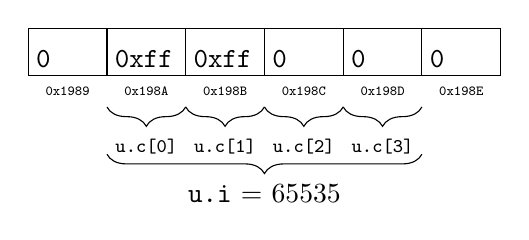
\begin{tikzpicture}
  [ 
    cell/.style={
       text width =8mm,
       text height=4mm, 
       draw=black, 
       inner sep  =1mm
    },
    ld/.style={
       draw=blue,
       shorten >=2pt,
       ->
    }
  ]
  \node (c00) at ( 0.0,1) [cell] {\ttfamily  0  };
  \node (c01) at ( 1.0,1) [cell] {\ttfamily 0xff};
  \node (c02) at ( 2.0,1) [cell] {\ttfamily 0xff};
  \node (c03) at ( 3.0,1) [cell] {\ttfamily  0  };
  \node (c04) at ( 4.0,1) [cell] {\ttfamily  0  };
  \node (c05) at ( 5.0,1) [cell] {\ttfamily  0  };

  \node (p00) at ( 0.0,0.5)      {\ttfamily \tiny 0x1989};
  \node (p01) at ( 1.0,0.5)      {\ttfamily \tiny 0x198A};
  \node (p02) at ( 2.0,0.5)      {\ttfamily \tiny 0x198B};
  \node (p03) at ( 3.0,0.5)      {\ttfamily \tiny 0x198C};
  \node (p04) at ( 4.0,0.5)      {\ttfamily \tiny 0x198D};
  \node (p05) at ( 5.0,0.5)      {\ttfamily \tiny 0x198E};
  
  \draw [decorate, decoration={brace,amplitude=7pt, mirror}, xshift=-0pt, yshift=0pt]
  		( 0.5, -0.3) -- ( 4.5, -0.3) node [midway, yshift=-0.5cm] 
		(braceArrayPreResize) {\texttt{u.i} = 65535};

  \draw [decorate, decoration={brace,amplitude=7pt, mirror}, xshift=-0pt, yshift=0pt]
  		( 0.5, 0.3) -- ( 1.5, 0.3) node [midway, yshift=-0.5cm] 
		(braceArrayPreResize) {\scriptsize \texttt{u.c[0]}};

  \draw [decorate, decoration={brace,amplitude=7pt, mirror}, xshift=-0pt, yshift=0pt]
  		( 1.5, 0.3) -- ( 2.5, 0.3) node [midway, yshift=-0.5cm] 
		(braceArrayPreResize) {\scriptsize \texttt{u.c[1]}};

  \draw [decorate, decoration={brace,amplitude=7pt, mirror}, xshift=-0pt, yshift=0pt]
  		( 2.5, 0.3) -- ( 3.5, 0.3) node [midway, yshift=-0.5cm] 
		(braceArrayPreResize) {\scriptsize \texttt{u.c[2]}};

  \draw [decorate, decoration={brace,amplitude=7pt, mirror}, xshift=-0pt, yshift=0pt]
  		( 3.5, 0.3) -- ( 4.5, 0.3) node [midway, yshift=-0.5cm] 
		(braceArrayPreResize) {\scriptsize \texttt{u.c[3]}};
\end{tikzpicture}
\end{center}
\end{tcolorbox}

Implizit bildet eine \mintinline{c}{union} also ein Interface auf eine Variable mit verschiedenen Typecasts.

\section{Automatisch numerierte Symbole: \mintinline{c}{enum}s}
\mintinline{c}{enum}s sind Aliase für \mintinline{c}{unsigned int}s, bei denen die einzelnen Zahlen neue Symbole zugewiesen bekommen. Die zugewiesenen Symbole können so gewählt werden, dass der Verwendungszweck klar wird. Syntaktisch lehnen sich \mintinline{c}{enum}s an \mintinline{c}{struct}s an; die einzelnen Elemente eines \mintinline{c}{enum}s werden aber durch Kommata getrennt, nicht durch Semikolons:

\begin{codebox}[Syntax: Deklaration einer \texttt{enum}]
\begin{minted}{c}
typedef enum {
  Symbol0, Symbol1, ...
} Name;
\end{minted}
\end{codebox}
\texttt{Symbol0} steht dann für den Wert \texttt{0}, \texttt{Symbol1} für \texttt{1} und so fort.

Betrachten Sie den folgenden Code: Es wird geprüft, welche von zwei Karten den Höheren Rang im Spiel hat, wobei \emph{Herz} als Trumpffarbe zählt. Sticht eine Karte \texttt{k1} eine andere Karte \texttt{k2}, so ist das Ergebnis \texttt{-1}; wenn \texttt{k2} den höheren Rang hat, wird \texttt{+1} zurückgegeben. Bei Gleichheit wird die Funktion zu \texttt{0} ausgewertet\footnote{Sie sehen hier eine Verwendung von \mintinline{c}{goto}. Wie erwähnt sollte der Gebrauch dieses Befehls sehr stark hinterfragt werden. An dieser Stelle führt die Alternative -- eine \mintinline{c}{if-else if}-Konstruktion mit verketteten Bedingungen -- jedoch zu einer weniger schnell erfassbaren Struktur. Versuchen Sie gerne als Übung, eine Funktion mit gleicher Wirkung ohne \mintinline{c}{goto} zu schreiben, und vergleichen Sie das Ergebnis.}.
\begin{codebox}[Beispiel: Deklaration einer \texttt{struct}]
\begin{minted}[linenos]{c}
typedef enum {Herz, Karo, Kreuz, Pik} Kartenfarbe;

typedef struct {
   int         Wert;
   Kartenfarbe Farbe;
} Karte;

int vergleicheKarten (Karte k1, Karte k2) {
  if   (k1.Farbe == Herz) {
    if (k2.Farbe == Herz) {goto vergleicheKartenWerte;}
    else                  {return -1;}
  }
  
  if   (k2.Farbe == Herz) {return  1;}
  
  vergleicheKartenWerte:
  if (k1.Wert == k2.Wert) {return 0;}
  else                    {return k1.Wert > k2.Wert  ?  -1  :  1;}
}
\end{minted}
\end{codebox}

Intern wird das Feld \texttt{Farbe} als \mintinline{c}{unsigned int} angelegt, und das Symbol \texttt{Herz} zum Wert \texttt{0} übersetzt. Es ist ebenso zulässig, \texttt{k1.Farbe == 0} zu prüfen oder eine Zuweisung \texttt{k2.Farbe = 3} zu machen. Jedoch ist mit der Vergabe von \mintinline{c}{enum}-Symbolen sofort ein Kontext gegeben, der den Code besser interpretierbar macht.

\section{C++}
\begin{plusbox}
In C++ sind \mintinline{c}{struct}s das zentrale Element; sie werden dort um viele Konzepte erweitert. Aus Feinheiten, die hier nicht behandelt werden können, benutzt man in C++ eher das Schlüsselwort \mintinline{c++}{class}, das im Wesentlichen dieselbe Wirkung hat wie das hier gezeigte \mintinline{c}{struct}.

Wir bilden alle \emph{Objekte} als solche \mintinline{c++}{class} ab und ordnen ihnen \emph{Methoden} zu, \ie Funktionen, die mit den Feldern einer \mintinline{c++}{class} arbeiten. Ein \emph{Objekt} ist eine nahezu beliebige gedankliche Einheit von Werten, die untereinander in einem funktionalen Zusammenhang stehen. \emph{Methoden} stehen nicht mehr \enquote{neben} der \mintinline{c++}{class}, sondern sind gänzlich in diese eingebunden. Über ein Schlüsselwort \mintinline{c++}{this} \enquote{sieht} die Methode alle Felder, die zu einer Instanz der \mintinline{c++}{class} gehören.

Klassen erlauben \emph{Zugriffskontrolle}, verbieten also das direkte Lesen und Schreiben von bestimmten Feldern. Nur die Methoden einer Klasse können alle Felder bearbeiten. Auf diese Weise soll ein versehentliches Ändern von Werten und damit das Entstehen von inkonsistenten (unsinnigen) Zuständen verhindern.

Weiter erlaubt C++ die Definition von \emph{Konstruktoren} und \emph{Destruktoren}, \ie Programmen, die automatisch aufgerufen werden, wenn eine Instanz der Klasse erzeugt wird, bzw. wenn sie das Ende ihrer Lebensdauer erreicht. Diese speziellen Methoden reservieren \idR Speicher für komplexere Strukturen bzw. geben diesen wieder frei.

Schließlich ist es in C++ auch möglich, eigene Operatoren zu definieren, und so direkt mit dem Symbol \texttt{+} zwei Instanzen einer Klasse zu addieren anstatt hierfür explizit eine Funktion aufrufen zu müssen.

Auch hier soll lediglich auf den Umfang des Themas hingewiesen und ein Anreiz geschaffen werden, den Kurs \emph{C++ und Qt} der Universität Regensburg zu besuchen.
\end{plusbox}